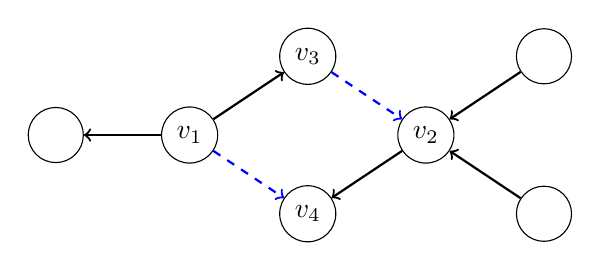
\begin{tikzpicture}
      \draw (-1.5, 0) node[draw = black, circle, minimum size = 0.7cm] (v1) {$v_1$};
      \draw (1.5, 0) node[draw = black, circle, minimum size = 0.7cm] (v2) {$v_2$};
      \draw (0, 1) node[draw = black, circle, minimum size = 0.7cm] (v3) {$v_3$};
      \draw (0, -1) node[draw = black, circle, minimum size = 0.7cm](v4) {$v_4$};
    %   \draw (-3, 1) node[draw = black, circle, minimum size = 0.7cm] (v5) {};
      \draw (-3.2, 0) node[draw = black, circle, minimum size = 0.7cm] (v6) {};
      \draw (3, 1) node[draw = black, circle, minimum size = 0.7cm] (v7) {};
      \draw (3, -1) node[draw = black, circle, minimum size = 0.7cm] (v8) {};
  
      \draw[->, thick, dashed, blue] (v1) -- (v4);
      \draw[->, thick, dashed, blue] (v3) -- (v2);
      \draw[->, thick] (v1) -- (v3);
    %   \draw[->, thick] (v5) -- (v1);
      \draw[->, thick] (v1) -- (v6);
      \draw[->, thick] (v2) -- (v4);
      \draw[->, thick] (v7) -- (v2);
      \draw[->, thick] (v8) -- (v2);
  \end{tikzpicture}